\documentclass{scrbook}


%!TEX root = thesis.tex

% Set german to default language and load english as well
\usepackage[english,ngerman]{babel}

% Set UTF8 as input encoding
\usepackage[utf8]{inputenc}

% Set T1 as font encoding
\usepackage[T1]{fontenc}
% Load a slightly more modern font
\usepackage{lmodern}
% Use the symbol collection textcomp, which is needed by listings.
\usepackage{textcomp}
% Load a better font for monospace.
\usepackage{courier}

% Set some options regarding the document layout. See KOMA guide
\KOMAoptions{%
  paper=a4,
  fontsize=12pt,
  parskip=half,
  headings=normal,
  BCOR=1cm,
  headsepline,
  DIV=12}

% do not align bottom of pages
\raggedbottom

% set style of captions
\setcapindent{0pt} % do not indent second line of captions
\setkomafont{caption}{\small}
\setkomafont{captionlabel}{\bfseries}
\setcapwidth[c]{0.9\textwidth}

% set the style of the bibliography
\bibliographystyle{alphadin}

% load extended tabulars used in the list of abbreviation
\usepackage{tabularx}

% load the color package and enable colored tables
\usepackage[table]{xcolor}

% define new environment for zebra tables
\newcommand{\mainrowcolors}{\rowcolors{1}{maincolor!25}{maincolor!5}}
\newenvironment{zebratabular}{\mainrowcolors\begin{tabular}}{\end{tabular}}
\newcommand{\setrownumber}[1]{\global\rownum#1\relax}
\newcommand{\headerrow}{\rowcolor{maincolor!50}\setrownumber1}

% add main color to section headers
\addtokomafont{chapter}{\color{maincolor}}
\addtokomafont{section}{\color{maincolor}}
\addtokomafont{subsection}{\color{maincolor}}
\addtokomafont{subsubsection}{\color{maincolor}}
\addtokomafont{paragraph}{\color{maincolor}}

% do not print numbers next to each formula
\usepackage{mathtools}
\mathtoolsset{showonlyrefs}
% left align formulas
\makeatletter
\@fleqntrue\let\mathindent\@mathmargin \@mathmargin=\leftmargini
\makeatother

% Allow page breaks in align environments
\allowdisplaybreaks

% header and footer
\usepackage{scrpage2}
\pagestyle{scrheadings}
\setkomafont{pagenumber}{\normalfont\sffamily\color{maincolor}}
\setkomafont{pageheadfoot}{\normalfont\sffamily}
\setheadsepline{0.5pt}[\color{maincolor}]

% German guillemets quotes
\usepackage[german=guillemets]{csquotes}

% load TikZ to draw diagrams
\usepackage{tikz}

% load additional libraries for TikZ
\usetikzlibrary{%
  automata,%
  positioning,%
}

% set some default options for TikZ -- in this case for automata
\tikzset{
  every state/.style={
    draw=maincolor,
    thick,
    fill=maincolor!18,
    minimum size=0pt
  }
}

% load listings package to typeset sourcecode
\usepackage{listings}

% set some options for the listings package
\lstset{%
  upquote=true,%
  showstringspaces=false,%
  basicstyle=\ttfamily,%
  keywordstyle=\color{keywordcolor}\slshape,%
  commentstyle=\color{commentcolor}\itshape,%
  stringstyle=\color{stringcolor}}

% enable german umlauts in listings
\lstset{
  literate={ö}{{\"o}}1
           {Ö}{{\"O}}1
           {ä}{{\"a}}1
           {Ä}{{\"A}}1
           {ü}{{\"u}}1
           {Ü}{{\"U}}1
           {ß}{{\ss}}1
}

% define style for pseudo code
\lstdefinestyle{pseudo}{language={},%
  basicstyle=\normalfont,%
  morecomment=[l]{//},%
  morekeywords={for,to,while,do,if,then,else},%
  mathescape=true,%
  columns=fullflexible}

% load the AMS math library to typeset formulas
\usepackage{amsmath}
\usepackage{amsthm}
\usepackage{thmtools}
\usepackage{amssymb}

% load the paralist library to use compactitem and compactenum environment
\usepackage{paralist}

% load varioref and hyperref to create nicer references using vref
\usepackage[ngerman]{varioref}
\PassOptionsToPackage{hyphens}{url} % allow line break at hyphens in URLs
\usepackage{hyperref}

% setup hyperref
\hypersetup{breaklinks=true,
            pdfborder={0 0 0},
            ngerman,
            pdfhighlight={/N},
            pdfdisplaydoctitle=true}

% Fix bugs in some package, e.g. listings and hyperref
\usepackage{scrhack}

% define german names for referenced elements
% (vref automatically inserts these names in front of the references)
\labelformat{figure}{Abbildung\ #1}
\labelformat{table}{Tabelle\ #1}
\labelformat{appendix}{Anhang\ #1}
\labelformat{chapter}{Kapitel\ #1}
\labelformat{section}{Abschnitt\ #1}
\labelformat{subsection}{Unterabschnitt\ #1}
\labelformat{subsubsection}{Unterunterabschnitt\ #1}

% define theorem environments
\declaretheorem[numberwithin=chapter,style=plain]{Theorem}
\labelformat{Theorem}{Theorem\ #1}

\declaretheorem[sibling=Theorem,style=plain]{Lemma}
\labelformat{Lemma}{Lemma\ #1}

\declaretheorem[sibling=Theorem,style=plain]{Korollar}
\labelformat{Korollar}{Korollar\ #1}

\declaretheorem[sibling=Theorem,style=definition]{Definition}
\labelformat{Definition}{Definition\ #1}

\declaretheorem[sibling=Theorem,style=definition]{Beispiel}
\labelformat{Beispiel}{Beispiel\ #1}

\declaretheorem[sibling=Theorem,style=definition]{Bemerkung}
\labelformat{Bemerkung}{Bemerkung\ #1}

%!TEX root = thesis.tex

% Use this file to define some macros you need in your thesis. A macro is a short command that inserts some mathematical symbols or texts you do not want to retype each time you need some. I recommend to use as many macros as possible, because you are able to change them later. For example if you use the same macro each time you need to give the formal semantics of an expression you can easily change the appearance of these brackets by updating the macro later on.

% Set of natural numbers
\newcommand{\N}{\mathbb{N}}

% The default epsilon does not look very nice
\let\epsilon\varepsilon

% If you need to use mathematical expressins like an epsilon in the section titles of your thesis you will end up with warnings that these special symbols cannot be included in the PDF favorites. The following macro uses the mathematical symbol during the text of the thesis and the string "Epsilon" in the PDF favorites.
\newcommand{\pdfepsilon}{\texorpdfstring{$\epsilon$}{Epsilon}}


% Set title and author used in the PDF meta data
\hypersetup{
  pdftitle={Spülbecken},
  pdfauthor={niemand}
}

% Depending on which of the following two color schemes you import your thesis will be in color or grayscale. I recommend to generate a colored version as a PDF and a grayscale version for printing.

%!TEX root = thesis.tex

% define color of example university
\xdefinecolor{exampleuniversity}{rgb}{1, 0.5, 0}

\colorlet{maincolor}{exampleuniversity}

\colorlet{stringcolor}{green!60!black}
\colorlet{commentcolor}{black!50}
\colorlet{keywordcolor}{maincolor!80!black}

\newcommand{\imagesuffix}{-color}
%\input{schema-gray}

\newcommand{\duedate}{\today}

\begin{document}
  \frontmatter
  %!TEX root = thesis.tex

\begin{titlepage}
  \thispagestyle{empty}

  \vskip1cm

  \pgfimage[height=2.5cm]{uni-logo-example\imagesuffix}
  
  \vskip2.5cm
  
  \LARGE
  
  \textbf{\sffamily\color{maincolor}Spülbecken}

  \textit{Kitchen Sinks}

  \normalfont\normalsize

  \vskip2em
  
  \textbf{\sffamily\color{maincolor}Masterarbeit}

  im Rahmen des Studiengangs \\
  \textbf{\sffamily\color{maincolor}Materialkunde} \\
  der Universität der Küchengeräte

  \vskip1em

  vorgelegt von \\
  \textbf{\sffamily\color{maincolor}Max Mustermann}

  \vskip1em
  
  ausgegeben und betreut von \\
  \textbf{\sffamily\color{maincolor}Prof. Prof. Dr. Dr. Erika Küchenhilfe}

  \vskip1em

  mit Unterstützung von\\
  Prof. Dr. Chefkoch 

  \vfill

  Küchendorf, den \duedate
\end{titlepage}

  %!TEX root = thesis.tex

\cleardoublepage
\thispagestyle{plain}
\vspace*{\fill}

\section*{Erklärung}

Hiermit erkläre ich an Eides statt, dass ich die vorliegende
Arbeit ohne unzulässige Hilfe Dritter und ohne die Benutzung anderer
als der angegebenen Hilfsmittel selbständig verfasst habe;
die aus anderen Quellen direkt oder indirekt übernommenen Daten und Konzepte
sind unter Angabe des Literaturzitats gekennzeichnet.

\vskip2cm

\rule{5cm}{0.4pt}\\
(Max Mustermann)\\
Musterhausen, den \duedate

  %!TEX root = thesis.tex

\cleardoublepage
\thispagestyle{plain}

\pdfbookmark{Spülbecken}{Spülbecken}
\paragraph{Kurzfassung}
Ein Spülbecken (ugs. auch Spüle) (in Österreich auch „die Abwasch“, in der Schweiz vorwiegend „Abwaschbecken“), ist meist in die Platte der Küchenarbeitsfläche eingelassen und wird zur Vorbereitung von Speisen (z. B. Reinigen von Obst, Salat oder Gemüse) und zur Säuberung von Geschirr und Küchenmaterialien benutzt. Der Unterschied zum Waschbecken ist hygienischer Natur, während umgangssprachlich diese häufig nicht mehr unterschieden werden.


\cleardoublepage
\thispagestyle{plain}

\foreignlanguage{english}{%
\pdfbookmark{Abstract}{abstract}
\paragraph{Abstract}
A sink—also known by other names including sinker, washbowl, hand basin and wash basin—is a bowl-shaped plumbing fixture used for washing hands, dishwashing, and other purposes. Sinks have taps (faucets) that supply hot and cold water and may include a spray feature to be used for faster rinsing. They also include a drain to remove used water; this drain may itself include a strainer and/or shut-off device and an overflow-prevention device. Sinks may also have an integrated soap dispenser.
}


  \cleardoublepage
  \phantomsection
  \pdfbookmark{Inhaltsverzeichnis}{tableofcontents}
  \markboth{Inhaltsverzeichnis}{}
  \tableofcontents

  \mainmatter
  %!TEX root = thesis.tex

\chapter{Einleitung}
Ein Spülbecken (ugs. auch Spüle) (in Österreich auch „die Abwasch“, in der Schweiz vorwiegend „Abwaschbecken“), ist meist in die Platte der Küchenarbeitsfläche eingelassen und wird zur Vorbereitung von Speisen (z. B. Reinigen von Obst, Salat oder Gemüse) und zur Säuberung von Geschirr und Küchenmaterialien benutzt. Der Unterschied zum Waschbecken ist hygienischer Natur, während umgangssprachlich diese häufig nicht mehr unterschieden werden. Während in Waschbecken beispielsweise auch mal Schmierstoffe verwendet werden, ist es eine subjektive Frage inwieweit man diese gemeinsam mit Lebensmitteln bearbeiten möchte. Schüttsteine gab es bereits im Mittelalter, zumeist jedoch nur in Burgen oder Schlössern. Der umgangssprachlich in manchen Regionen (z. B. dem Rheinland) übliche Ausdruck Spülstein für das Spülbecken stammt noch hiervon ab.

Das Spülbecken zählt gemeinsam mit Herd und Kühlschrank zur Grundausstattung einer modernen Küche. Die Spüle ist zumeist mit einer Küchenarmatur ausgestattet und somit der zentrale Punkt, um die Küche mit heißem und kaltem Wasser zu versorgen. Im fränkischen Sprachraum wird das zweite Becken auch als Abfleibecken bezeichnet.


  \chapter{Inhalt}

\section{Spülenkonzepte}
Man unterscheidet zwischen Ein- und Mehrbecken-Spülen. Letztere verfügen über ein kleineres Zusatzbecken und/oder ein zweites vollwertiges Hauptbecken, um parallele Arbeitsgänge wie das Ausgießen von Resten oder das Waschen von Gemüse zu ermöglichen. Da die meisten Haushalte über einen Geschirrspüler verfügen, ist zum komfortablen Reinigen größerer Gegenstände, z. B. Backblechen, Schneidbrettern oder Woks, ein geräumiges Hauptbecken mit großer Beckendiagonale besonders vorteilhaft. Häufig werden Spülbecken mit einer Abtropffläche[1] kombiniert, um abtropfendes Wasser in das Spülbecken zurückzuführen.

Rundbecken-Spülen sind zumeist als Einbecken-Spülen mit vergleichsweise kleinen Spülbecken konzipiert. Eckspülen sind spezielle Lösungen für Eckunterschränke. \cite{moore}\cite{MopOverview}

Spülbecken müssen in Deutschland mit einem Überlauf ausgestattet sein, um dem versehentlichen Fluten der Küche vorzubeugen; in anderen Staaten sind auch Spülen ohne Überlauf zugelassen.\cite{scala}\cite{rltl}

Für die Gastronomie sind Spülbecken in der DIN 66075-5 (Gastro-Norm: Einrichtungen für die Gastronomie; Spülbecken, Maße; Ausgabe 1975-07) genormt.


\section{Materialien}
Edelstahl ist der populärste Werkstoff für Spülbecken, der seit den 1950er Jahren in verschiedenen Material-Spezifikationen (z. B. DIN 1.4301) zum Einsatz kommt. Neben der klassischen glatten Oberfläche in unterschiedlichsten Veredelungen werden auch Spülen aus geprägtem Edelstahl, z. B. mit Leinen-Struktur, angeboten, die die Empfindlichkeit des Materials gegenüber Kratzern halbwegs kaschiert. Die Produktion von einfacheren Edelstahl-Spülen erfolgt durch Tiefziehen von Edelstahlblechen, anspruchsvollere Produkte entstehen durch Zusammenfügen mehrerer tiefgezogener Komponenten, aber auch durch Verschweißen von Blechzuschnitten. \cite{bitkom}\cite{Leucker02}

Seit Beginn der 1980er Jahre gibt es Küchenspülen aus hochwertigen Verbundwerkstoffen. Sie werden in vielen Farben und Formen angeboten. Hochwertige Produkte sind zumeist ausgesprochen kratzfest und pflegeleicht und halten Temperaturen bis 280 °C sowie allen küchenüblichen Beanspruchungen (z. B. stark färbende Lebensmittel oder Säuren) stand. Moderne Produktionsverfahren ermöglichen auch filigrane Formen, die mit anderen Werkstoffen nicht zu realisieren sind.

Keramik und Steinzeug sind traditionelle Werkstoffe, die seit vielen Jahrzehnten auch für die Herstellung von Küchenspülen eingesetzt werden.
Keramik-Spüle mit Zusatzbecken, Tropffläche, umhängbarer Edelstahl-Schale und verschiebbarem Schneidbrett aus Sicherheitsglas

Ein ebenfalls früher häufiger verwendeter Werkstoff ist Terrazzo, der heute jedoch nur noch für besonders exklusive Becken verwendet wird. Nachteilig ist das verhältnismäßig große Gewicht, das eine entsprechend stabile Unterkonstruktion nötig macht.

Naturstein ist als Material für Spülbecken weitgehend bedeutungslos geworden da viele Steinmaterialien nicht widerstandsfähig genug sind (z. B. Marmor) oder nicht mehr heutigen hygienischen Ansprüchen entsprechen (z. B. der Flüssigkeiten aufsaugende Sandstein).

Glas wird zumeist mit anderen Werkstoffen kombiniert. In den meisten Fällen werden Edelstahl-Becken mit einem horizontalen Arbeitsbereich aus Glas verbunden. \cite{RltlConv}

Emaillierter Stahl hat als Spülen-Werkstoff nur noch geringe Bedeutung. Er steht für die Anfänge farbiger Küchen-Spülen, die seit den Achtziger Jahren durch komfortablere und strapazierfähigere Produkte aus Verbundwerkstoff oder farbiger Keramik verdrängt wurden. \cite{codecommit}


\begin{figure}[ht]
	\centering
  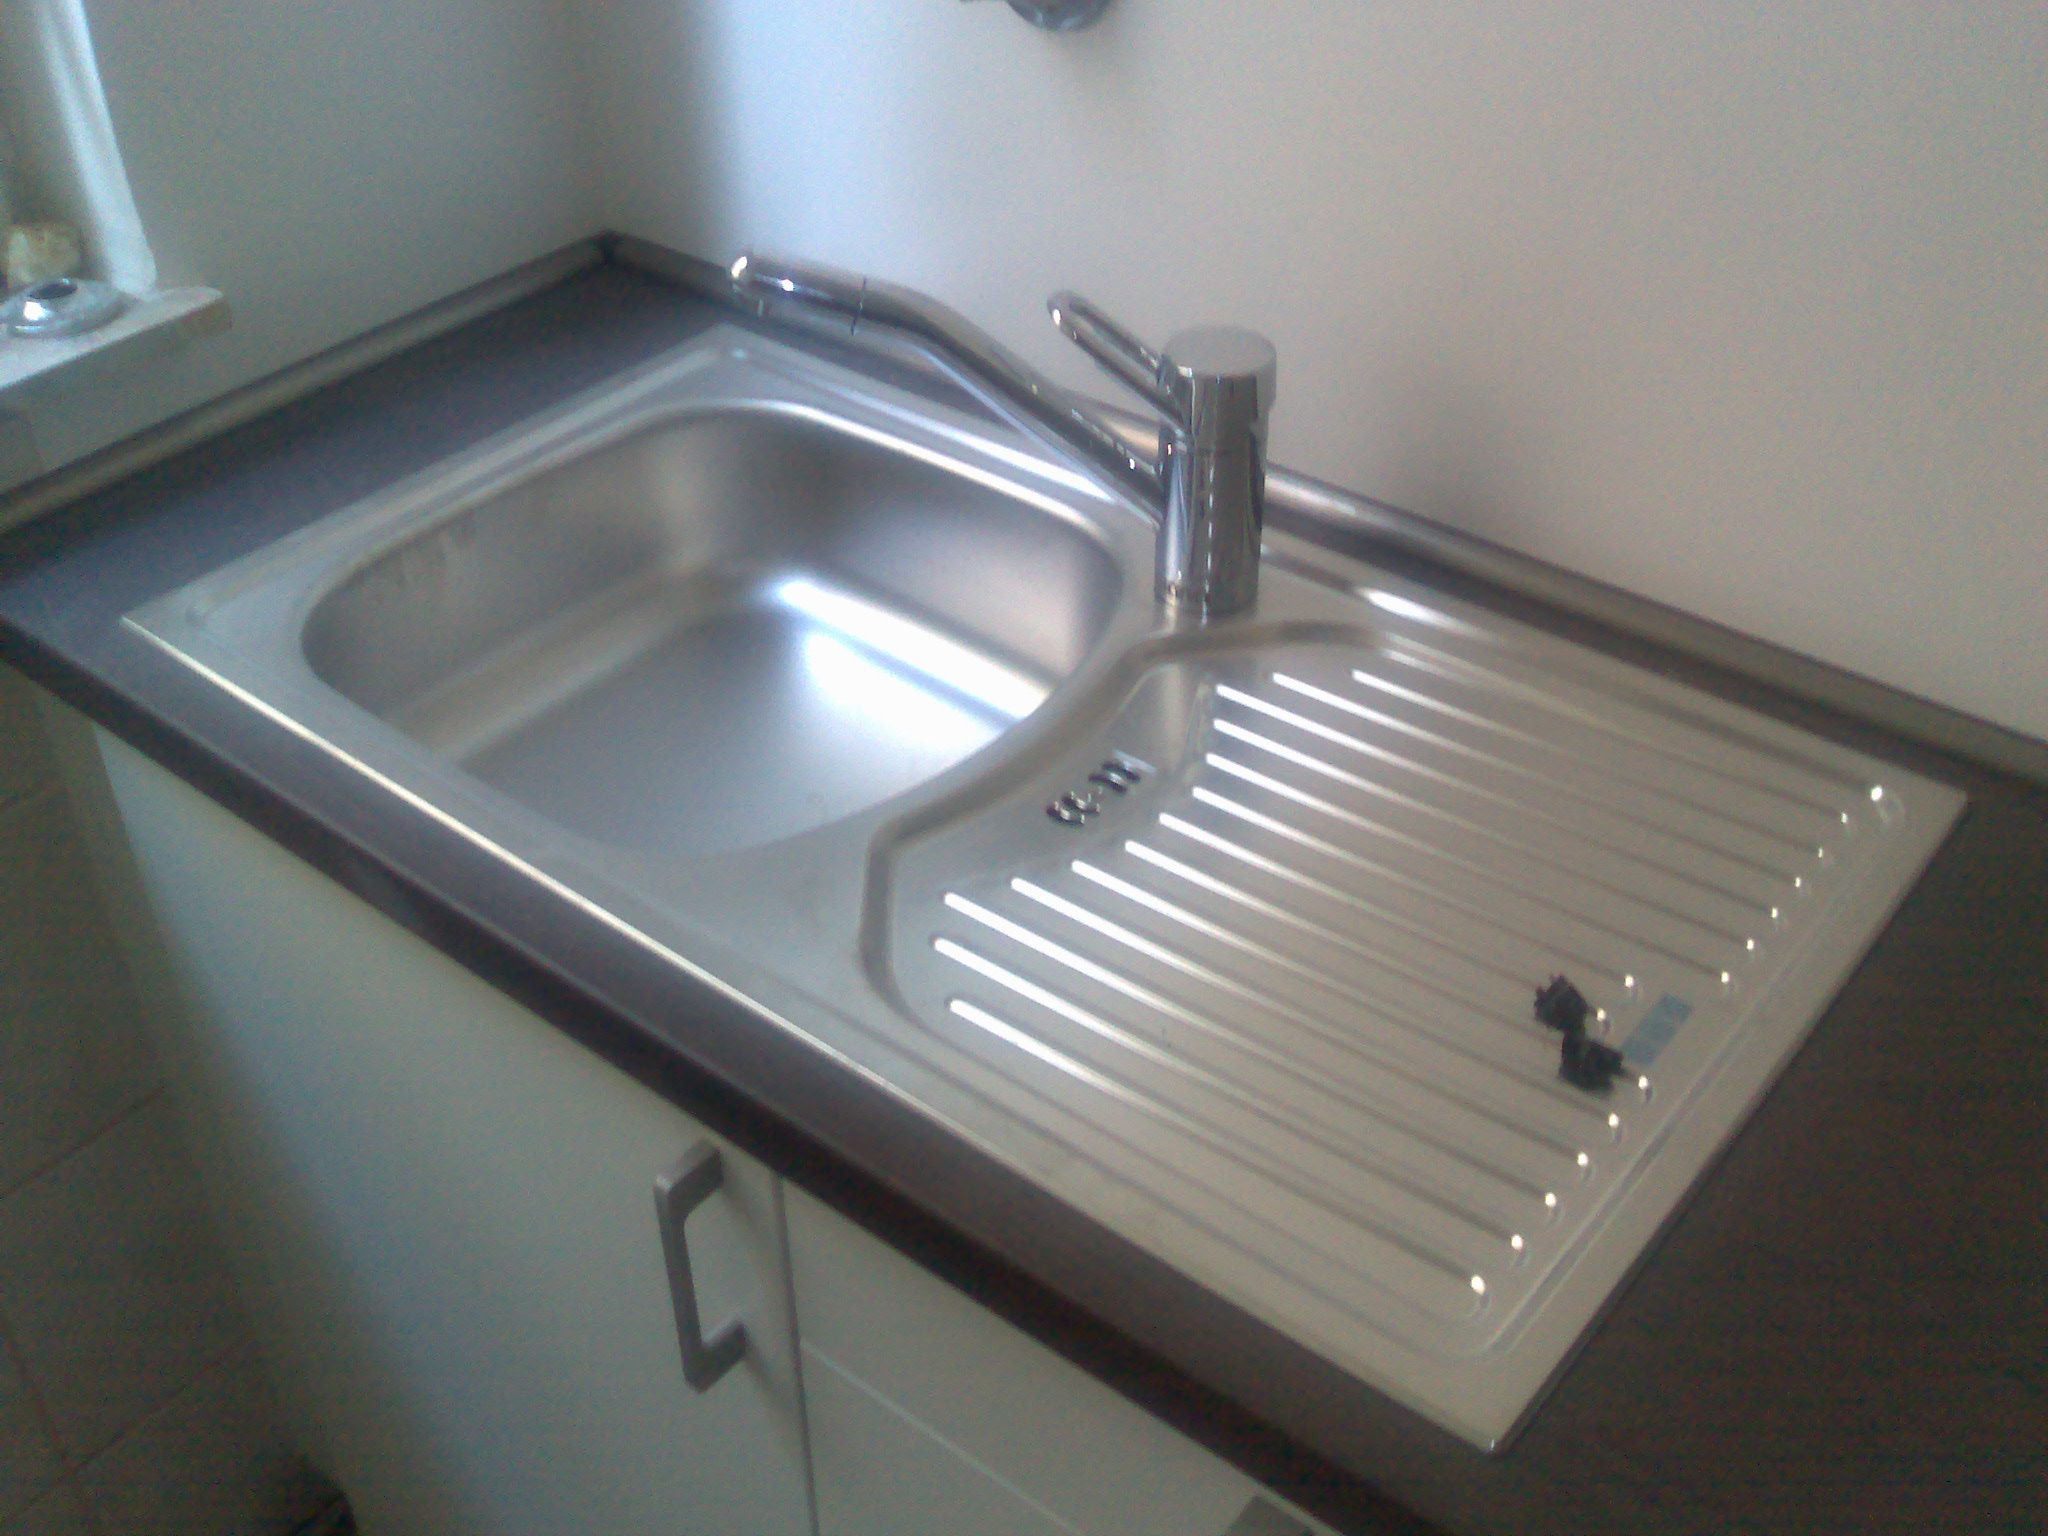
\includegraphics[width=0.9\textwidth]{Spuelbecken.jpg}
	\caption{Spülbecken mit Abtropffläche}
	\label{fig1}
\end{figure}


\begin{figure}[ht]
	\centering
  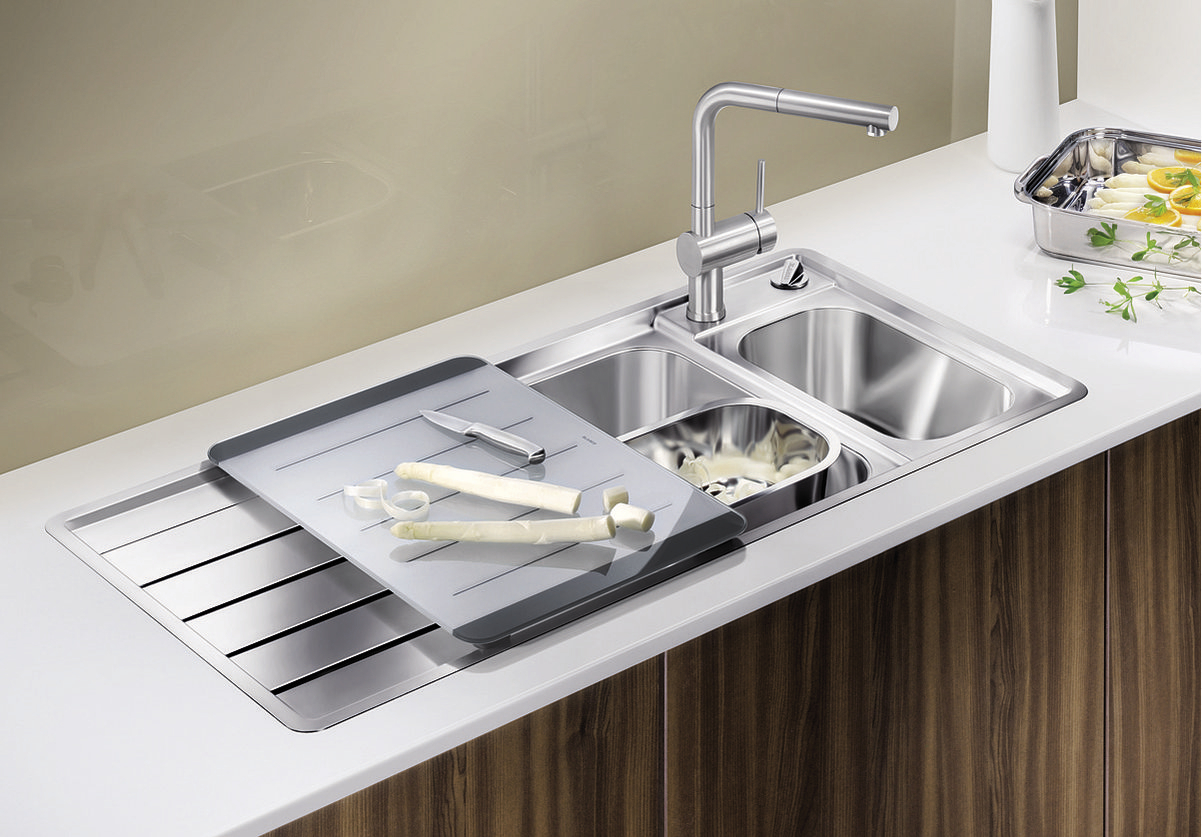
\includegraphics[width=0.9\textwidth]{Spuelbecken2.jpg}
	\caption{
Edelstahl-Spüle mit Zusatzbecken, Tropffläche und verschiebbarem Schneidbrett aus Sicherheitsglas}
	\label{fig1}
\end{figure}


%  \include{grundlagen}
%  \include{konzept}
%  \include{evaluation}
%  \include{fazit}

  \appendix

%  \include{appendix}

  \backmatter

  \cleardoublepage
  \phantomsection
  \pdfbookmark{Abbildungsverzeichnis}{listoffigures}
  \listoffigures
%
%  \cleardoublepage
%  \phantomsection
%  \pdfbookmark{Tabellenverzeichnis}{listoftables}
%  \listoftables

  \cleardoublepage
  \phantomsection
  \pdfbookmark{Definitions- und Theoremverzeichnis}{listoftheorems}
  \renewcommand{\listtheoremname}{Definitions- und Theoremverzeichnis}
  \listoftheorems[ignoreall,show={Lemma,Theorem,Korollar,Definition}]

%  \include{abkuerzungen}

  \cleardoublepage
  \phantomsection
  \pdfbookmark{Literaturverzeichnis}{bibliography}
  \bibliography{literature}
\end{document}
